\documentclass[a4paper,12pt]{report}
%\usepackage[backend=biber]{biblatex}
\usepackage[backend=bibtex]{biblatex}
\addbibresource{reference.bib}
\usepackage[hidelinks]{hyperref}
\usepackage{float}
\usepackage{graphicx}
\usepackage{listings}
\usepackage[utf8]{inputenc}
\usepackage{etoolbox}
\usepackage{fullpage}
\renewcommand*\contentsname{Indice}
\renewcommand{\lstlistingname}{Listato}
\renewcommand{\figurename}{Figura}
\renewcommand{\bibname}{Bibliografia}
\usepackage{setspace}
\usepackage{parskip}
\usepackage{amsmath}

% un po' di estetica...
\usepackage{fancyhdr}
\pagestyle{fancy}
\setlength{\headsep}{0.35in}
\let\MakeUppercase\relax

% blocchi di codice
\usepackage{listings}
\lstset{
	breaklines=true, 
	frame=single, 
	numbers=left,
	tabsize=2,
	basicstyle=\scriptsize,
	showstringspaces=false,
	language=C++
}

\setlength{\parindent}{2em}
\setlength{\parskip}{0.5em}
\renewcommand{\baselinestretch}{1.5}

\fancyhf{} % clear all fields
\fancyfoot[C]{\thepage}

\frenchspacing

\newcommand{\mychapter}[2]{
    \setcounter{chapter}{#1}
    \setcounter{section}{0}
    \chapter*{#2}
    \addcontentsline{toc}{chapter}{#2}
}

\begin{document}

\begin{titlepage}
\noindent
    \vspace*{5mm}
	\begin{minipage}[t]{0.15\textwidth}
	    \vspace*{5mm}
		\vspace{-3.5mm}{
\includegraphics[scale=1.8]{../img/logo_bicocca.png}}
	\end{minipage}
	\hspace{1cm}
	\begin{minipage}[t]{0.9\textwidth}
	      \vspace*{5mm}
		{
			\setstretch{1.42}
			{\textsc{Università degli Studi di Milano - Bicocca} } \\
			\textbf{Scuola di Scienze} \\
			\textbf{Dipartimento di Informatica, Sistemistica e Comunicazione} \\
			\textbf{Corso di Laurea Magistrale in Informatica} \\
			\par
		}
	\end{minipage}
	
	\vspace{42mm}

\begin{center}
    {\LARGE{
	    	\setstretch{2}
            \textbf{
            	Metodi del Calcolo Scientifico - Progetto 2 \\ 
            	Compressione di immagini tramite la DCT \\ }
    }}        
\end{center}

\vspace{40mm}
	
	
	\begin{flushright}
		\setstretch{1.3}
		\large{Alberici Federico - 808058\\} 
		\large{Bettini Ivo Junior - 806878\\} 
		\large{Cocca Umberto - 807191\\} 
		\large{Traversa Silvia - 816435} 
	\end{flushright}
	
	\vspace{15mm}
	\begin{center}
		{\large{\bf Anno Accademico 2019 - 2020}}
	\end{center}


\renewcommand{\baselinestretch}{1.5}

\end{titlepage}

\tableofcontents

\mychapter{0}{Introduzione}
In questa relazione vengono presentate e discusse le modalità di implementazione della DCT (dall'inglese Discrete Cosine Transform), ovvero la più diffusa funzione che provvede alla compressione spaziale.\\
Nella prima parte viene confrontata la versione nativa delle DCT implementata in questo progetto con alcune varianti fast (FFT), studiandone il costo computazionale.\\   %"Nativa" della DCT con alcune varianti conosciute, studiandone il costo computazionale.\\
Nella seconda parte viene documentato un semplice tool per applicare su immagini in toni di grigio, tramite un approccio di compressione di tipo jpeg (senza utilizzare una matrice di quantizzazione), utilizzando tutte le funzioni DCT2 implementate, tenendo di default quella fast.

\noindent È possibile trovare il listato dei codici alla seguente \href{https://gitlab.com/AlbezJelt/dct2}{\textbf{repository}}.


\mychapter{1}{Analisi DCT}

\section{Discrete Cosine Transform}
Una DCT esprime una sequenza finita di punti in termini di una somma di funzioni coseno oscillanti a diverse frequenze. Ad oggi è una delle tecniche di trasformazione più utilizzate nella Teoria dei segnali e nella compressione dei dati, in particolare nei media digitali (audio, video, radio ecc..).\\
In queste applicazioni infatti la maggior parte delle informazioni significative tendono a essere concentrate in poche componenti a bassa frequenza della DCT. Questo permette di comprimere a piacere il dato scartando le componenti ad alta frequenza (compressione lossy).

\section{DCT e IDCT}
La DCT-II è probabilmente la forma più utilizzata, infatti viene indicata come "la DCT".\\
\[C_k = \alpha_k \sum_{i=0}^{N-1} V_i\cos \left[\frac{\pi \left(2i + 1\right) k }{2N}\right] \quad i = 0, \dots, N-1 \quad e \quad \alpha_k = \begin{cases} 1/\sqrt{N}, & \mbox{se } k\mbox{ = 0} \\ \sqrt{2/N}, & \mbox{se } \mbox{\(1 \leq k \leq N - 1\)} \end{cases}\]\\\\
La sua inversa è la DCT-III e per questo viene indicata come "l'inversa della DCT" o "IDCT".\\
\[V_i = \sum_{k=0}^{N-1} \alpha_k C_k \cos \left[\frac{\pi \left(2i + 1\right) k }{2N}\right] \quad k = 0, \dots, N-1 \quad e \quad \alpha_k = \begin{cases} 1/\sqrt{N}, & \mbox{se } k\mbox{ = 0} \\ \sqrt{2/N}, & \mbox{se } \mbox{\(1 \leq k \leq N - 1\)} \end{cases}\]\\\\

\noindent Entrambe le funzioni effettuano N somme per calcolare la k-esima componente di un vettore di N componenti, determinando un costo computazionale \( O(N^2)\).

\subsection*{Implementazione}
Per l'implementazione è stato utilizzato C++, sfruttando la libreria open-source Eigen (\url{https://eigen.tuxfamily.org/}) per semplificare la gestione dei dati.\\
\begin{lstlisting}[caption={Funzione di calcolo DCT},captionpos=b]
	void DCT2::DCT(Eigen::VectorXd &_v)
	{
	
		const Eigen::VectorXd _v_copy = _v;
		const int N = _v.size();
		double ak = 1.0 / sqrt(N);
		double ck = 0;
	
		for (int k = 0; k < N; k++)
		{
			ck = 0;
			for (int i = 0; i < N; i++)
			{
				ck += cos((2.0 * i + 1.0) * k * M_PI / (2.0 * N)) * _v_copy(i);
			}
			_v(k) = ak * ck;
			if (k == 0)
			{
				ak = sqrt(2.0) / sqrt(N);
			}
		}
	}
\end{lstlisting}
\hfill \break
\begin{lstlisting}[caption={Funzione di calcolo IDCT},captionpos=b]
void DCT2::IDCT(Eigen::VectorXd &_c)
{
    const Eigen::VectorXd _c_copy = _c;
    const int N = _c.size();
    double ak = 0;
    double vi = 0;

    for (int i = 0; i < N; i++)
    {
        vi = 0;
        ak = 1.0 / sqrt(N);
        for (int k = 0; k < N; k++)
        {
            vi += cos((2.0 * i + 1.0) * k * M_PI / (2.0 * N)) * _c_copy(k) * ak;
            if (k == 0)
            {
                ak = sqrt(2.0) / sqrt(N);
            }
        }
        _c(i) = vi;
    }
}
\end{lstlisting}

\section{DCT2 e IDCT2}
La DCT2 è una trasformazione a due dimensioni, ottenuta semplicemente applicando la DCT mono-dimensionale prima per righe e poi per colonne (o viceversa).\\
La definizione della DCT bi-dimensionale per una matrice A di dimensione \textit{m} x \textit{n} in input è:\\
\begin{align*}
C_{kl} = \alpha_k \alpha_l \sum_{i=0}^{m-1} \sum_{j=0}^{n-1}&A_{ij} \cos \left[\frac{\pi \left(2i + 1\right) k }{2m}\right] \cos \left[\frac{\pi \left(2j + 1\right) l }{2n}\right],\\
&con \quad 0 \leq k \leq m - 1, \quad 0 \leq l \leq n - 1,\\
&\alpha_k = \begin{cases} 1/\sqrt{m}, & \mbox{se } i\mbox{ = 0} \\ \sqrt{2/m}, & \mbox{se } \mbox{\(1 \leq i \leq m - 1\)} \end{cases} \quad e \quad \alpha_l = \begin{cases} 1/\sqrt{n}, & \mbox{se } j\mbox{ = 0} \\ \sqrt{2/n}, & \mbox{se } \mbox{\(1 \leq j \leq n - 1\)} \end{cases}
\end{align*}
L'inversa di tale trasformazione è la IDCT2, ottenuta applicando IDCT alle due dimensioni.

\subsection*{Implementazione}
Anche in questo caso Eigen è stato utilizzato per mantenere la struttura dati tramite un oggetto \textit{Eigen::MatrixXd}. L'implementazione non sfrutta direttamente la definizione, ma computa la DCT2/IDCT2 prima sulle righe e poi sulle colonne della matrice in input. Inoltre, essendo l'elaborazione di ogni vettore indipendente dalle altre, è possibile parallelizzarne la computazione. La direttiva \textit{\# pragma omp parallel for} prima dei due cicli abilita la computazione concorrente della DCT sulle due dimensioni della matrice in input. \\
Dunque tale calcolo comporta l'esecuzione di una routine DCT su N righe e M colonne di una matrice, determinando un costo computazionale di:\\
\[ 
  \begin{cases} 
   O(N^2) O(N+M) = O(N^3) & \textit{se DCT di tipo II o III} \\
   O(N\log{N}) O(N+M) = O(N^2\log{N}) & \textit{se DCT versione fast (FCT)} 
  \end{cases}
\]
\hfill \break
\hfill \break
\hfill \break
\hfill \break
\begin{lstlisting}[caption={Funzione di calcolo DCT2},captionpos=b]
	Eigen::MatrixXd DCT2::DCT2_mt(Eigen::MatrixXd &_m)
	{
		Eigen::MatrixXd out = _m;
	
	// DCT su righe
	#pragma omp parallel for
		for (int i = 0; i < out.rows(); i++)
		{
			Eigen::VectorXd row = out.row(i);
			DCT(row);
			out.row(i) = row;
		}
	
	// DCT su colonne
	#pragma omp parallel for
		for (int i = 0; i < out.cols(); i++)
		{
			Eigen::VectorXd col = out.col(i);
			DCT(col);
			out.col(i) = col;
		}
	
		return out;
	}
\end{lstlisting}
\hfill \break
\begin{lstlisting}[caption={Funzione di calcolo IDCT2},captionpos=b]
	Eigen::MatrixXd DCT2::IDCT2_mt(Eigen::MatrixXd &_m)
	{
		Eigen::MatrixXd out = _m;
	
	// IDCT su righe
	#pragma omp parallel for
		for (int i = 0; i < out.rows(); i++)
		{
			Eigen::VectorXd row = out.row(i);
			IDCT(row);
			out.row(i) = row;
		}
	
	// IDCT su colonne
	#pragma omp parallel for
		for (int i = 0; i < out.cols(); i++)
		{
			Eigen::VectorXd col = out.col(i);
			IDCT(col);
			out.col(i) = col;
		}
	
		return out;
	}
\end{lstlisting}
\newpage

\section{Varianti DCT}
Esistono diverse varianti della DCT che riducono la complessità a \(O(NlogN)\). Tali metodi sono conosciuti come \textit{fast DCT} o \textit{FCT} in quanto appunto migliorano notevolmente il costo computazionale.\\Di seguito vengono citate due delle più comuni.

\subsubsection*{Fast DCT di Lee}
Descritta da Byeong Gi Lee \cite{Lee} nel 1984 è uno degli algoritmi fast DCT per \(2^m\) punti più comune. Utilizza una struttura ricorsiva dove la trasformazione DCT è decomposta in una parte pari e una dispari. Queste parti sono a loro volta decomposte nello stesso modo finchè non sono abbastanza piccole (m=1) da essere calcolate tramite valutazione diretta \cite{LAGERSTRM2001DesignAI}.

\subsubsection*{Fast DCT FFT}
Invece di applicare direttamente la formula DCT (o scomporla come mostrato da Lee) è possibile fattorizzare la computazione in modo simile alla \textit{fast Fourier transform} (FFT). Gli algoritmi basati sull'\textit{algoritmo di Cooley-Tukey} \cite{10.2307/2003354} per \(2^m\) punti sono i più comuni, ma qualunque altro algoritmo FFT è applicabile. Per esempio l'\textit{algoritmo FFT di Bluestein} (o \textit{algoritmo chirp-z}) permette di computare per una qualunque dimensione.\\

\noindent Gli algoritmi fast utilizzati nei confronti e test successivi provengono dal Project Nayuki \cite{nayuki}, modificati in modo da essere compatibili con gli oggetti Eigen. La versione FFT, in base alla dimensione in input, utilizza i due algoritmi sopra citati.\\
Come riportato dall'autore "non è difficile utilizzare una FFT per computare una fast DCT che elabori in tempo \(O(N\log{N})\), ma tale approccio introduce un piccolo fattore costante di penalità in tempo e spazio per memorizzare e computare numeri ridondanti".\\Gli algoritmi sono reperibili con una serie di Unit test che ne provano il corretto funzionamento.

\section{Confronto}
I dati utilizzati per generare i grafici seguenti sono stati raccolti applicando i vari algoritmi DCT2 su matrici random di dimensione fissata. Per ogni dimensione il tempo risultante è una media risultante da \textit{X} esecuzioni degli algoritmi, eseguiti finchè il tempo medio calcolato non si discostasse più da una certa soglia \textit{dist} per un determinato numero \textit{round} di iterazioni.

\subsubsection*{Dimensioni potenze di 2}
\begin{figure}[H]
\centering
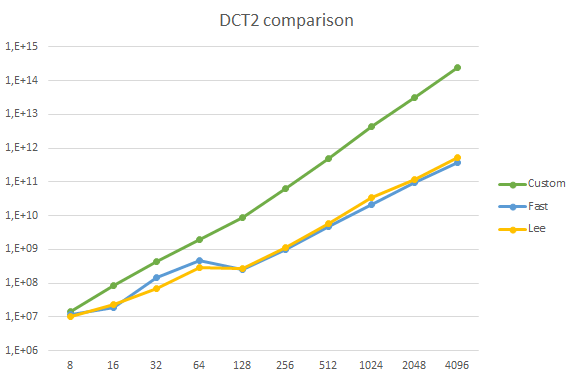
\includegraphics[width=0.77\linewidth]{../img/comparison.png}
\caption{\textit{Confronto DCT2 custom, Fast DCT di Lee e Fast DCT FFT}}
%\label{fig:2}
\end{figure}
\begin{center}
	\begin{tabular}{ |p{4cm}||p{2cm}|p{2cm}|p{2.5cm}|  }
		\hline
		\multicolumn{4}{|c|}{Vincoli} \\
		\hline
		Dimensione matrice& dist [ms] & round & time\_limit [s]\\
		\hline
		8 - 256   & 100    &5&   3600\\
		512 - 2048&   500  & 5   &3600\\
		4096 &500 & 2&  3600\\
		\hline
	\end{tabular}
\end{center}
\hfill \break
\hfill \break
Per poter rappresentare graficamente il confronto fra l'algoritmo di DCT2 da noi implementato (\textit{Custom}), e la versione DCT2 dell'algoritmo fast della libreria Lee (\textit{Lee}) e l'algoritmo che sfrutta la fast Fourier transform (\textit{Fast}) è stato utilizzato un grafico a linee con indicatori, ponendo sull'asse delle ascisse la dimensioni delle matrice quadrate (sono state utilizzate dimensioni in potenza di 2 per poter eseguire il codice di Lee) e sulle ordinate il tempo impiegato, espresso in scala logaritmica. \\
Si può notare chiaramente che la crescita del tempo impiegato dall'algoritmo Custom è esponenziale rispetto all'andamento similare che hanno gli algoritmi Fast e Lee. 

\subsubsection*{Altre dimensioni}
Valori fissi \(dist=100ms\), \(round=5\) e \(time\_limit=1800s\).
\begin{figure}[H]
\centering
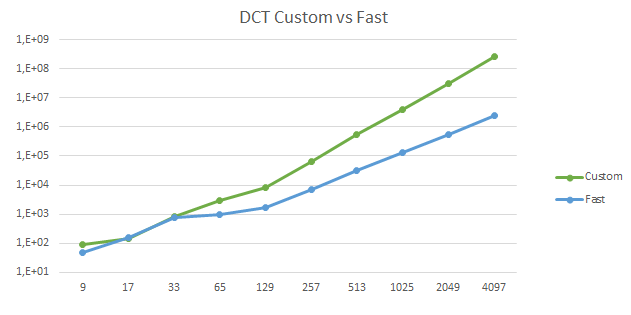
\includegraphics[width=0.77\linewidth]{../img/customvsfast.png}
\caption{\textit{Confronto DCT2 custom e Fast DCT}}
%\label{fig:2}
\end{figure}

\noindent Tale grafico dimostra che, anche senza il vincolo imposto dall'algoritmo di Lee sulla dimensione della matrice, i valori ottenuti con la \textit{DCT2 custom} e la \textit{fast DCT} mantengono lo stesso andamento con matrici di dimensioni incrementali. 


\mychapter{2}{Test con immagini}
Nella seconda parte del progetto l'interfaccia grafica è stata scritta tramite QT, una libreria multipiattaforma per lo sviluppo di programmi che utilizzano un'interfaccia (attraverso l'uso di widget) che si basa sul linguaggio C++ (motivo per il quale abbiamo deciso di utilizzarla).
\bigskip

\noindent Il programma utilizza le seguenti classi da noi implementate:
\begin{itemize}
\item \textbf{main.cpp}, la quale si occupa di eseguire l'intero corpo del programma;
\item \textbf{Compress.cpp}, che data una matrice \textit{x} crea iterativamente delle sottomatrici. Queste saranno poi passate alla libreria \textit{Fast DCT} per eseguire la compressione e ottenere come risultato finale l'immagine compressa. Inoltre, abbiamo aggiunto la possibilità di eseguire questa operazione anche attraverso la \textit{libreria di Lee} e la \textit{custom DCT2}.
\item \textbf{mainwindow.cpp}, classe che gestisce tutti gli aspetti e i trigger della interfaccia grafica;
\item \textbf{my\_qlabel.cpp}, classe di supporto che permette di visualizzare graficamente la quantità di dettaglio perso dell'immagine tenendo premuto sulla figura. La scelta di implementare questa classe è data dal fatto che con determinati parametri (come si potrà notare nella sezione Risultati) non è possibile notare a occhio nudo la differenza del risultato ottenuto rispetto all'immagine originale.
\end{itemize}

\section{Esecuzione del programma}
Una volta avviato il programma, è possibile caricare l'immagine .bmp dal filesystem attraverso un apposito tasto e inserire i valori di F e d. Una volta inseriti i parametri, tramite il pulsante \textit{Process} viene chiamato il metodo \textit{on\_parameters\_clicked()}, che dopo aver controllato se F e d rispettano tutti i vincoli (F positivo, d compreso fra 0 e 2F - 2), trasforma con la funzione \textit{pixmapToMatrix()} l'immagine in una matrice e la invia alla classe \textit{Compress.cpp}. In essa l'immagine viene divisa in blocchi e a ognuno di questi viene applicata la DCT2, restituendo poi una matrice che viene passata alla funzione \textit{matrixToPixmap()} per poter essere visualizzata in output nell'interfaccia grafica.
\bigskip

\noindent In particolare la classe \textit{Compress.cpp} prende in input una matrice di interi e i parametri F e d e restituisce in output una nuova matrice di interi. Al suo interno, la matrice di input viene trasformata in formato double e viene eseguito un troncamento per poter scartare gli "avanzi". Iterativamente, per ogni blocco quadrato F x F applichiamo la DCT2 e poi restituiamo la matrice nel formato int (arrotondando i valori double all'intero più vicino, mettendo a 0 i valori negativi e a 255 quelli maggiori di 255). 

\begin{figure}[H]
\centering
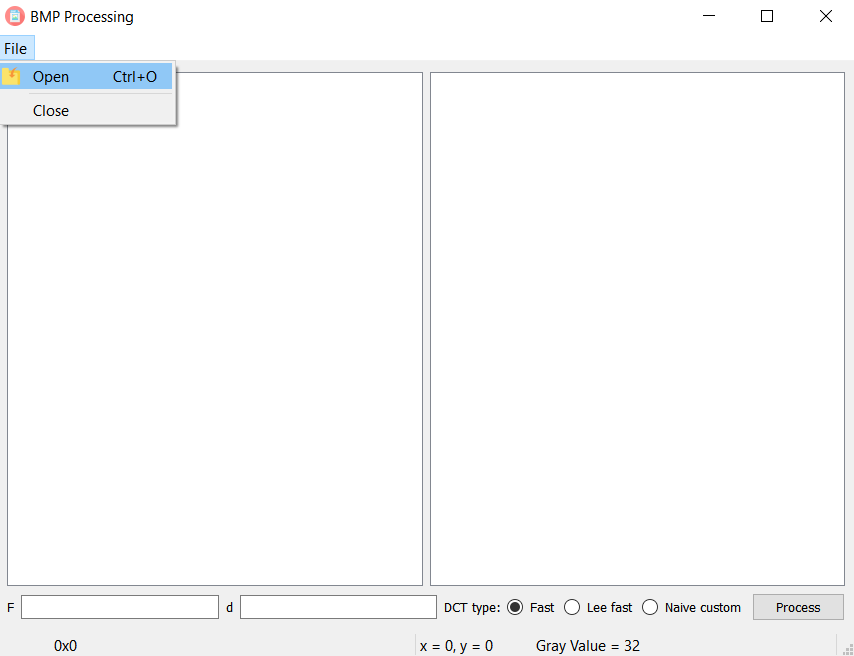
\includegraphics[width=0.7\linewidth]{../img/open.png}
\caption{\textit{Finestra di caricamento immagine da filesystem}}
\end{figure}

\newpage
\section{Risultati}
Il programma è stato testato sulle immagini di prova fornite e sono stati sperimentati diversi valori dei parametri \textit{F} e \textit{d}, utilizzando la libreria \textit{Fast DCT}.

\noindent L'immagine \textit{bridge.bmp} ha dimensione 2749 x 4049, impostando come parametri  \textit{F} = 200 e \textit{d} = 100 non è visibile alcuna differenza nell'immagine compressa.

\begin{figure}[H]
\centering
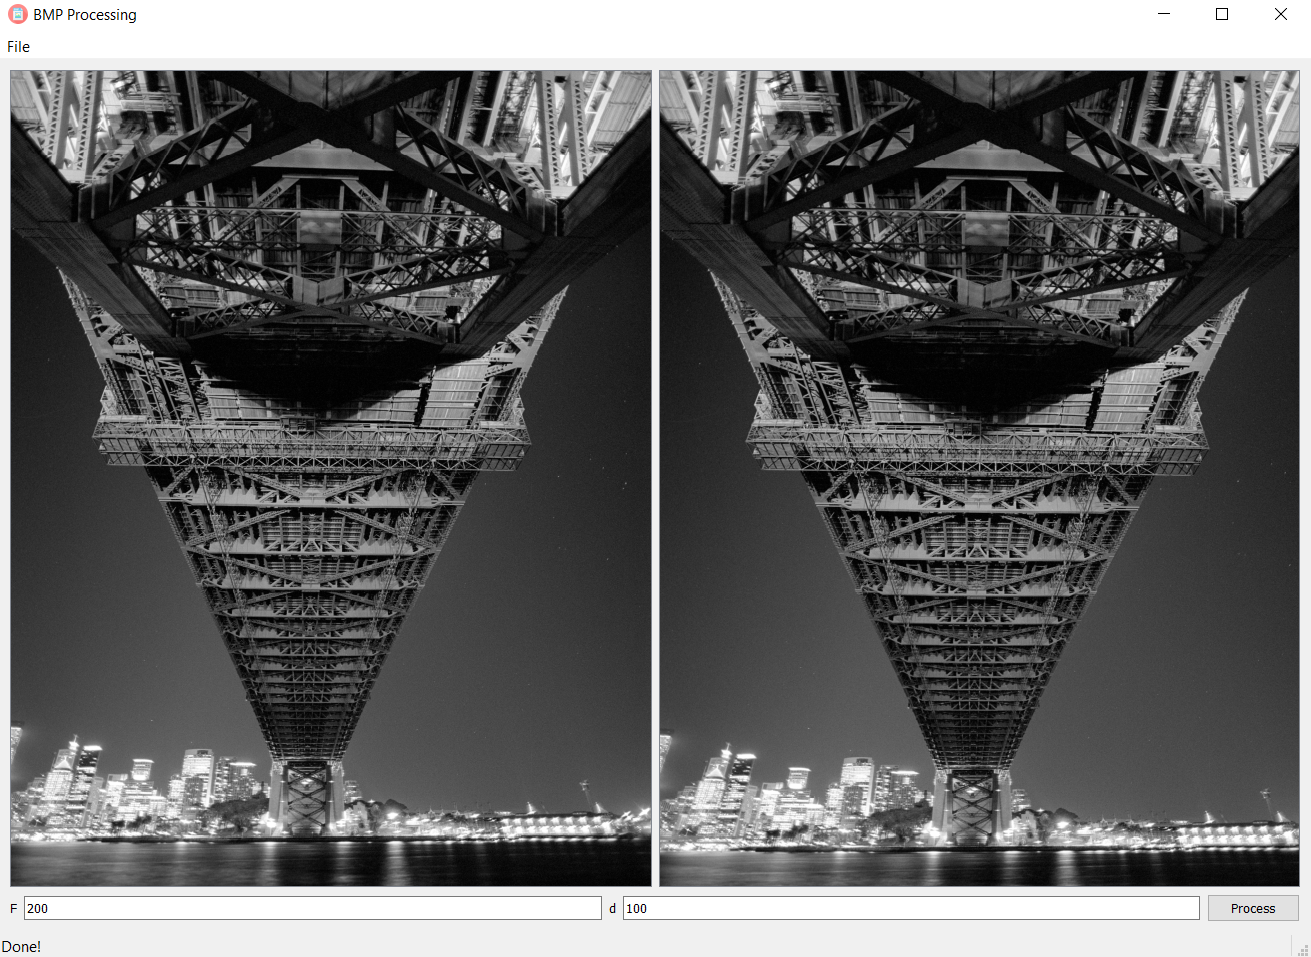
\includegraphics[width=0.65\linewidth]{../img/bridge_200_100.png}
\caption{\textit{bridge.bmp con F = 200 e d = 100}}
\end{figure}

\noindent Fissando il valore \textit{F} e diminuendo il valore del parametro \textit{d}, portandolo a 7, eliminando un gran numero di frequenze, sono visibili gli artefatti legati alla perdita di dettaglio.

\begin{figure}[H]
\centering
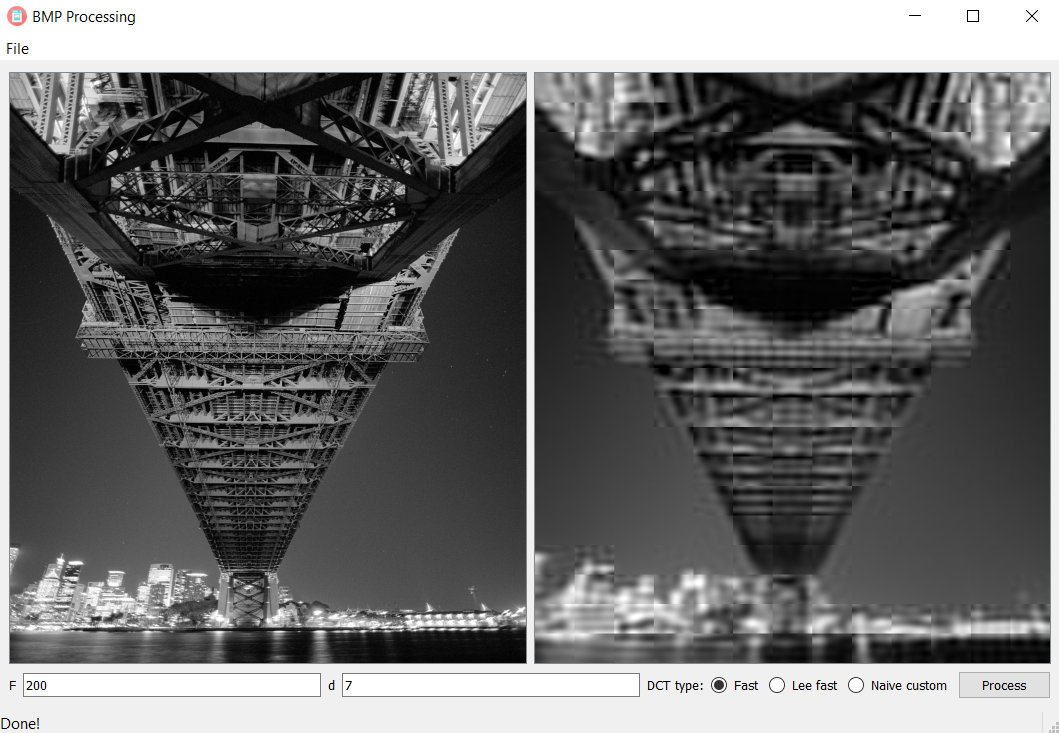
\includegraphics[width=0.65\linewidth]{../img/bridge_200_7.png}
\caption{\textit{bridge.bmp con F = 200 e d = 7}}
\end{figure}

\noindent Con l'immagine \textit{deer.bmp}, di dimensione 4043x2641 abbiamo voluto sperimentare con un valore di \textit{F} maggiore, pari a 250, e con valori di \textit{d} bassi.
Impostando \textit{d} = 50 l'immagine risulta lievemente sgranata.
\bigskip

\begin{figure}[H]
\centering
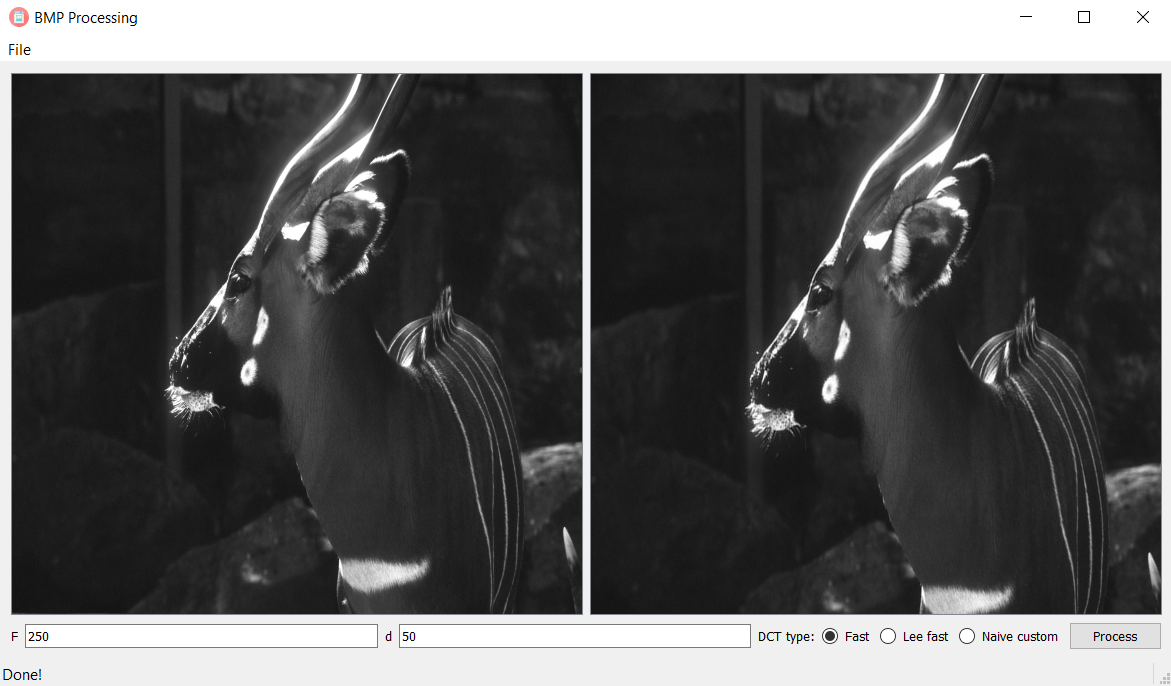
\includegraphics[width=0.75\linewidth]{../img/bambi_250_50.png}
\caption{\textit{deer.bmp con F = 250 e d = 50}}
\end{figure}

\noindent Abbassando il valore di \textit{d} a 9 sono visibili gli artefatti causati dalla perdita di dettaglio.
\bigskip

\begin{figure}[H]
\centering
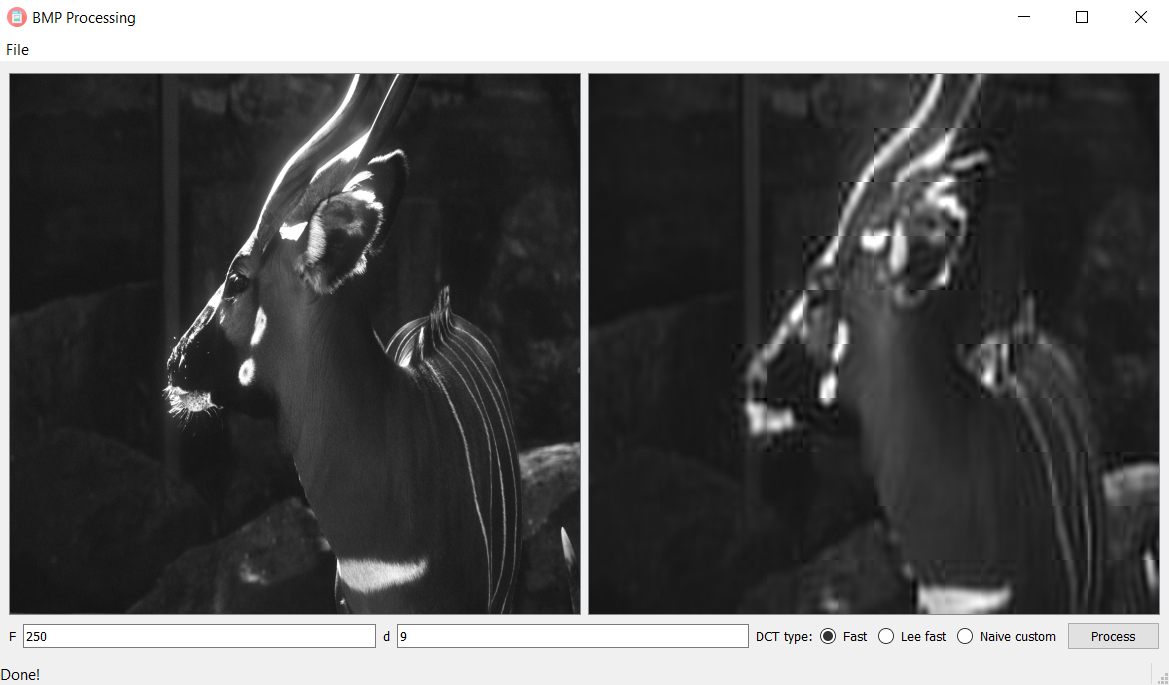
\includegraphics[width=0.75\linewidth]{../img/bambi_250_9.png}
\caption{\textit{deer.bmp con F = 250 e d = 9}}
\end{figure}

\newpage
\noindent Per l'immagine \textit{cathedral.bmp} (2000x3008) abbiamo voluto testare valori di \textit{F} piccoli con valori di \textit{d} relativamente vicini.
Ponendo \textit{F} = 20 e \textit{d} = 15 otteniamo un'immagine che non sembra differire dall'originale se non per una luminosità maggiore.

\begin{figure}[H]
\centering
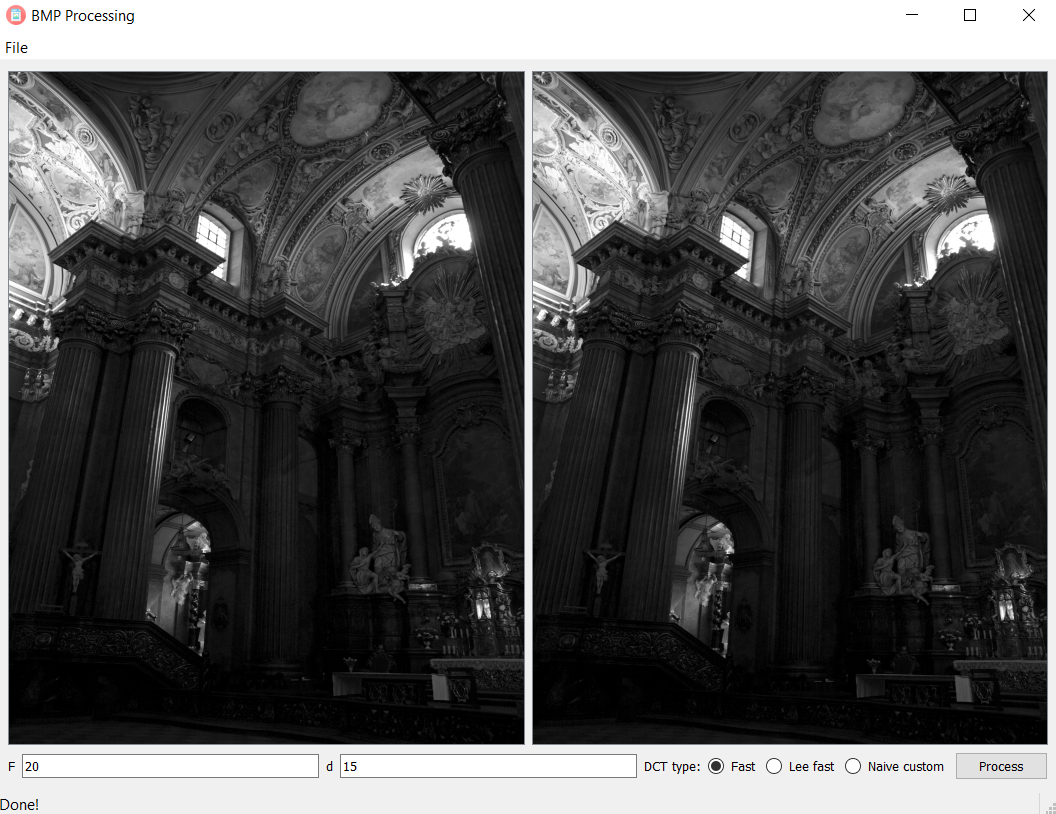
\includegraphics[width=0.65\linewidth]{../img/cathedral_20_15.png}
\caption{\textit{cathedral.bmp con F = 20 e d = 15}}
\end{figure}

\noindent Abbiamo successivamente impostato \textit{F} = 10 e abbiamo assegnato a \textit{d} un valore maggiore, 17. L'immagine risulta pressoché identica.

\begin{figure}[H]
\centering
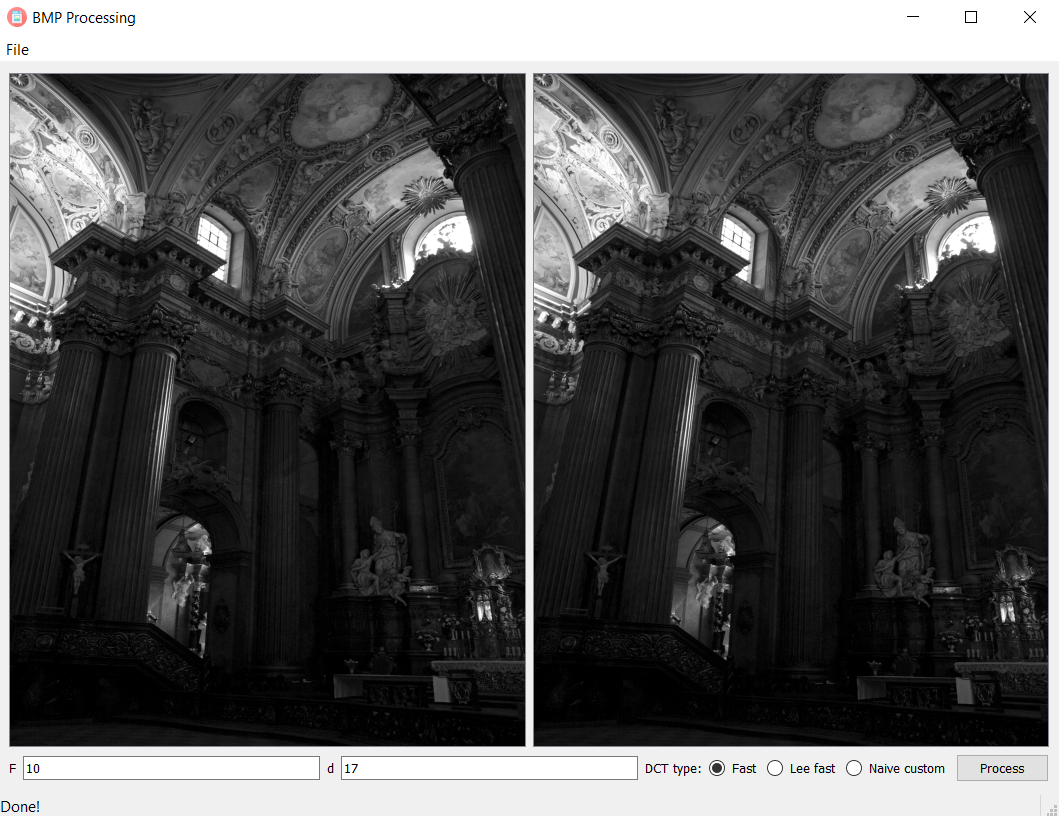
\includegraphics[width=0.65\linewidth]{../img/cathedral_10_17.png}
\caption{\textit{cathedral.bmp con F = 10 e d = 17}}
\end{figure}

\newpage

\noindent Abbiamo testato i casi limite su un'immagine scaricata da noi. Abbiamo assegnato a \textit{F} un valore casuale (in questo caso 10) e a \textit{d} il valore 0. In questo modo abbiamo dimostrato che vengono eliminate tutte le frequenze.

\begin{figure}[H]
\centering
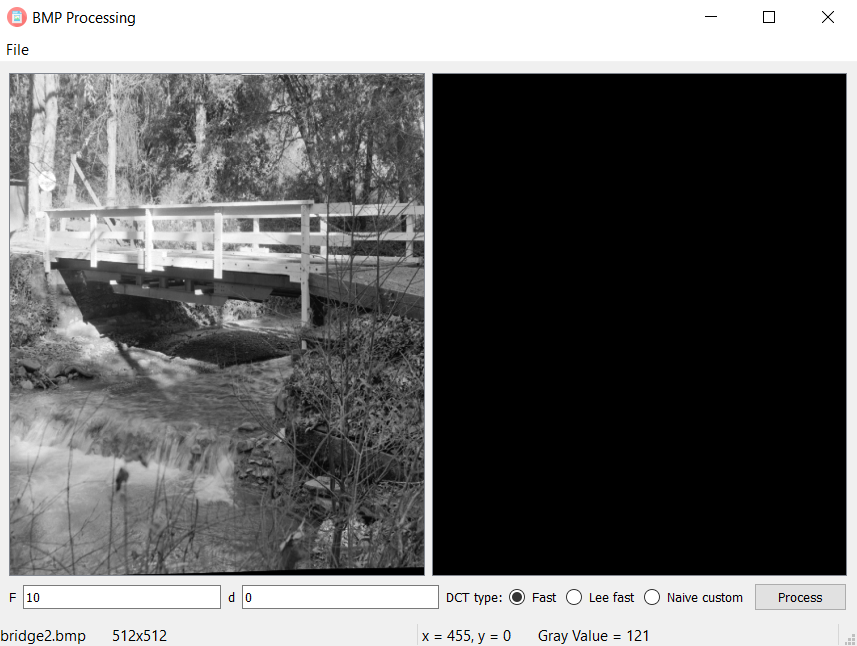
\includegraphics[width=0.65\linewidth]{../img/bridge2_10_0.png}
\caption{\textit{bridge2.bmp con F = 10 e d = 0}}
\end{figure}

\noindent In questo secondo caso, ponendo \textit{d} = 2F - 2 (in questo caso 18) viene eliminata solo la frequenza più alta.

\begin{figure}[H]
\centering
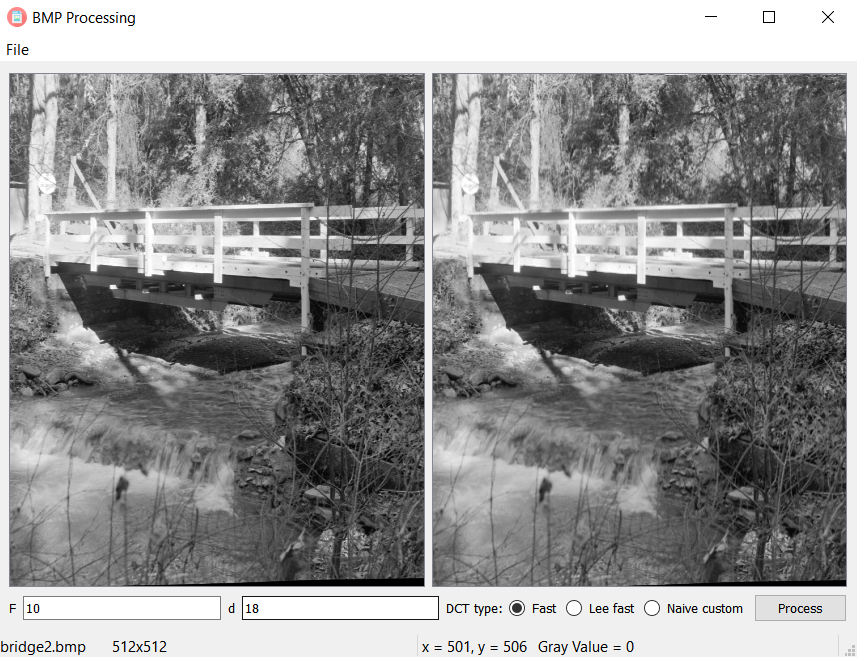
\includegraphics[width=0.65\linewidth]{../img/bridge2_10_18.png}
\caption{\textit{bridge2.bmp con F = 10 e d = 18}}
\end{figure}
\printbibliography

\end{document}